\Class{Psion}
{Resist all you like. I have ways of making you think.}{Dechares, Dwarven inquisitor}

The psion learns the Way, a philosophy of mental discipline, to become master of his will, or innate mental power. Most aspiring psions seek out an instructor, a master of the Way. Most Athasian cities contain psionic academies where students receive instructions in exchange for money or loyal service.

\PsychicTable{The Psion}{
1 & +0 & +0 & +0 & +2 & Bonus feat, discipline & 2 & 3 & 1st \\
2 & +1 & +0 & +0 & +3 &  & 6 & 5 & 1st \\
3 & +1 & +1 & +1 & +3 &  & 11 & 7 & 2nd \\
4 & +2 & +1 & +1 & +4 &  & 17 & 8 & 2nd \\
5 & +2 & +1 & +1 & +4 & Bonus feat & 25 & 11 & 3rd \\
6 & +3 & +2 & +2 & +5 &  & 35 & 13 & 3rd \\
7 & +3 & +2 & +2 & +5 &  & 46 & 15 & 4th \\
8 & +4 & +2 & +2 & +6 &  & 58 & 17 & 4th \\
9 & +4 & +3 & +3 & +6 &  & 72 & 19 & 5th \\
10 & +5 & +3 & +3 & +7 & Bonus feat & 88 & 21 & 5th \\
11 & +5 & +3 & +3 & +7 &  & 106 & 22 & 6th \\
12 & +6/+1 & +4 & +4 & +8 &  & 126 & 24 & 6th \\
13 & +6/+1 & +4 & +4 & +8 &  & 147 & 25 & 7th \\
14 & +7/+2 & +4 & +4 & +9 &  & 170 & 27 & 7th \\
15 & +7/+2 & +5 & +5 & +9 & Bonus feat & 195 & 28 & 8th \\
16 & +8/+3 & +5 & +5 & +10 &  & 221 & 30 & 8th \\
17 & +8/+3 & +5 & +5 & +10 &  & 250 & 31 & 9th \\
18 & +9/+4 & +6 & +6 & +11 &  & 280 & 33 & 9th \\
19 & +9/+4 & +6 & +6 & +11 &  & 311 & 34 & 9th \\
20 & +10/+5 & +6 & +6 & +12 & Bonus feat & 343 & 36 & 9th}

\begin{figure}[t!]
\centering
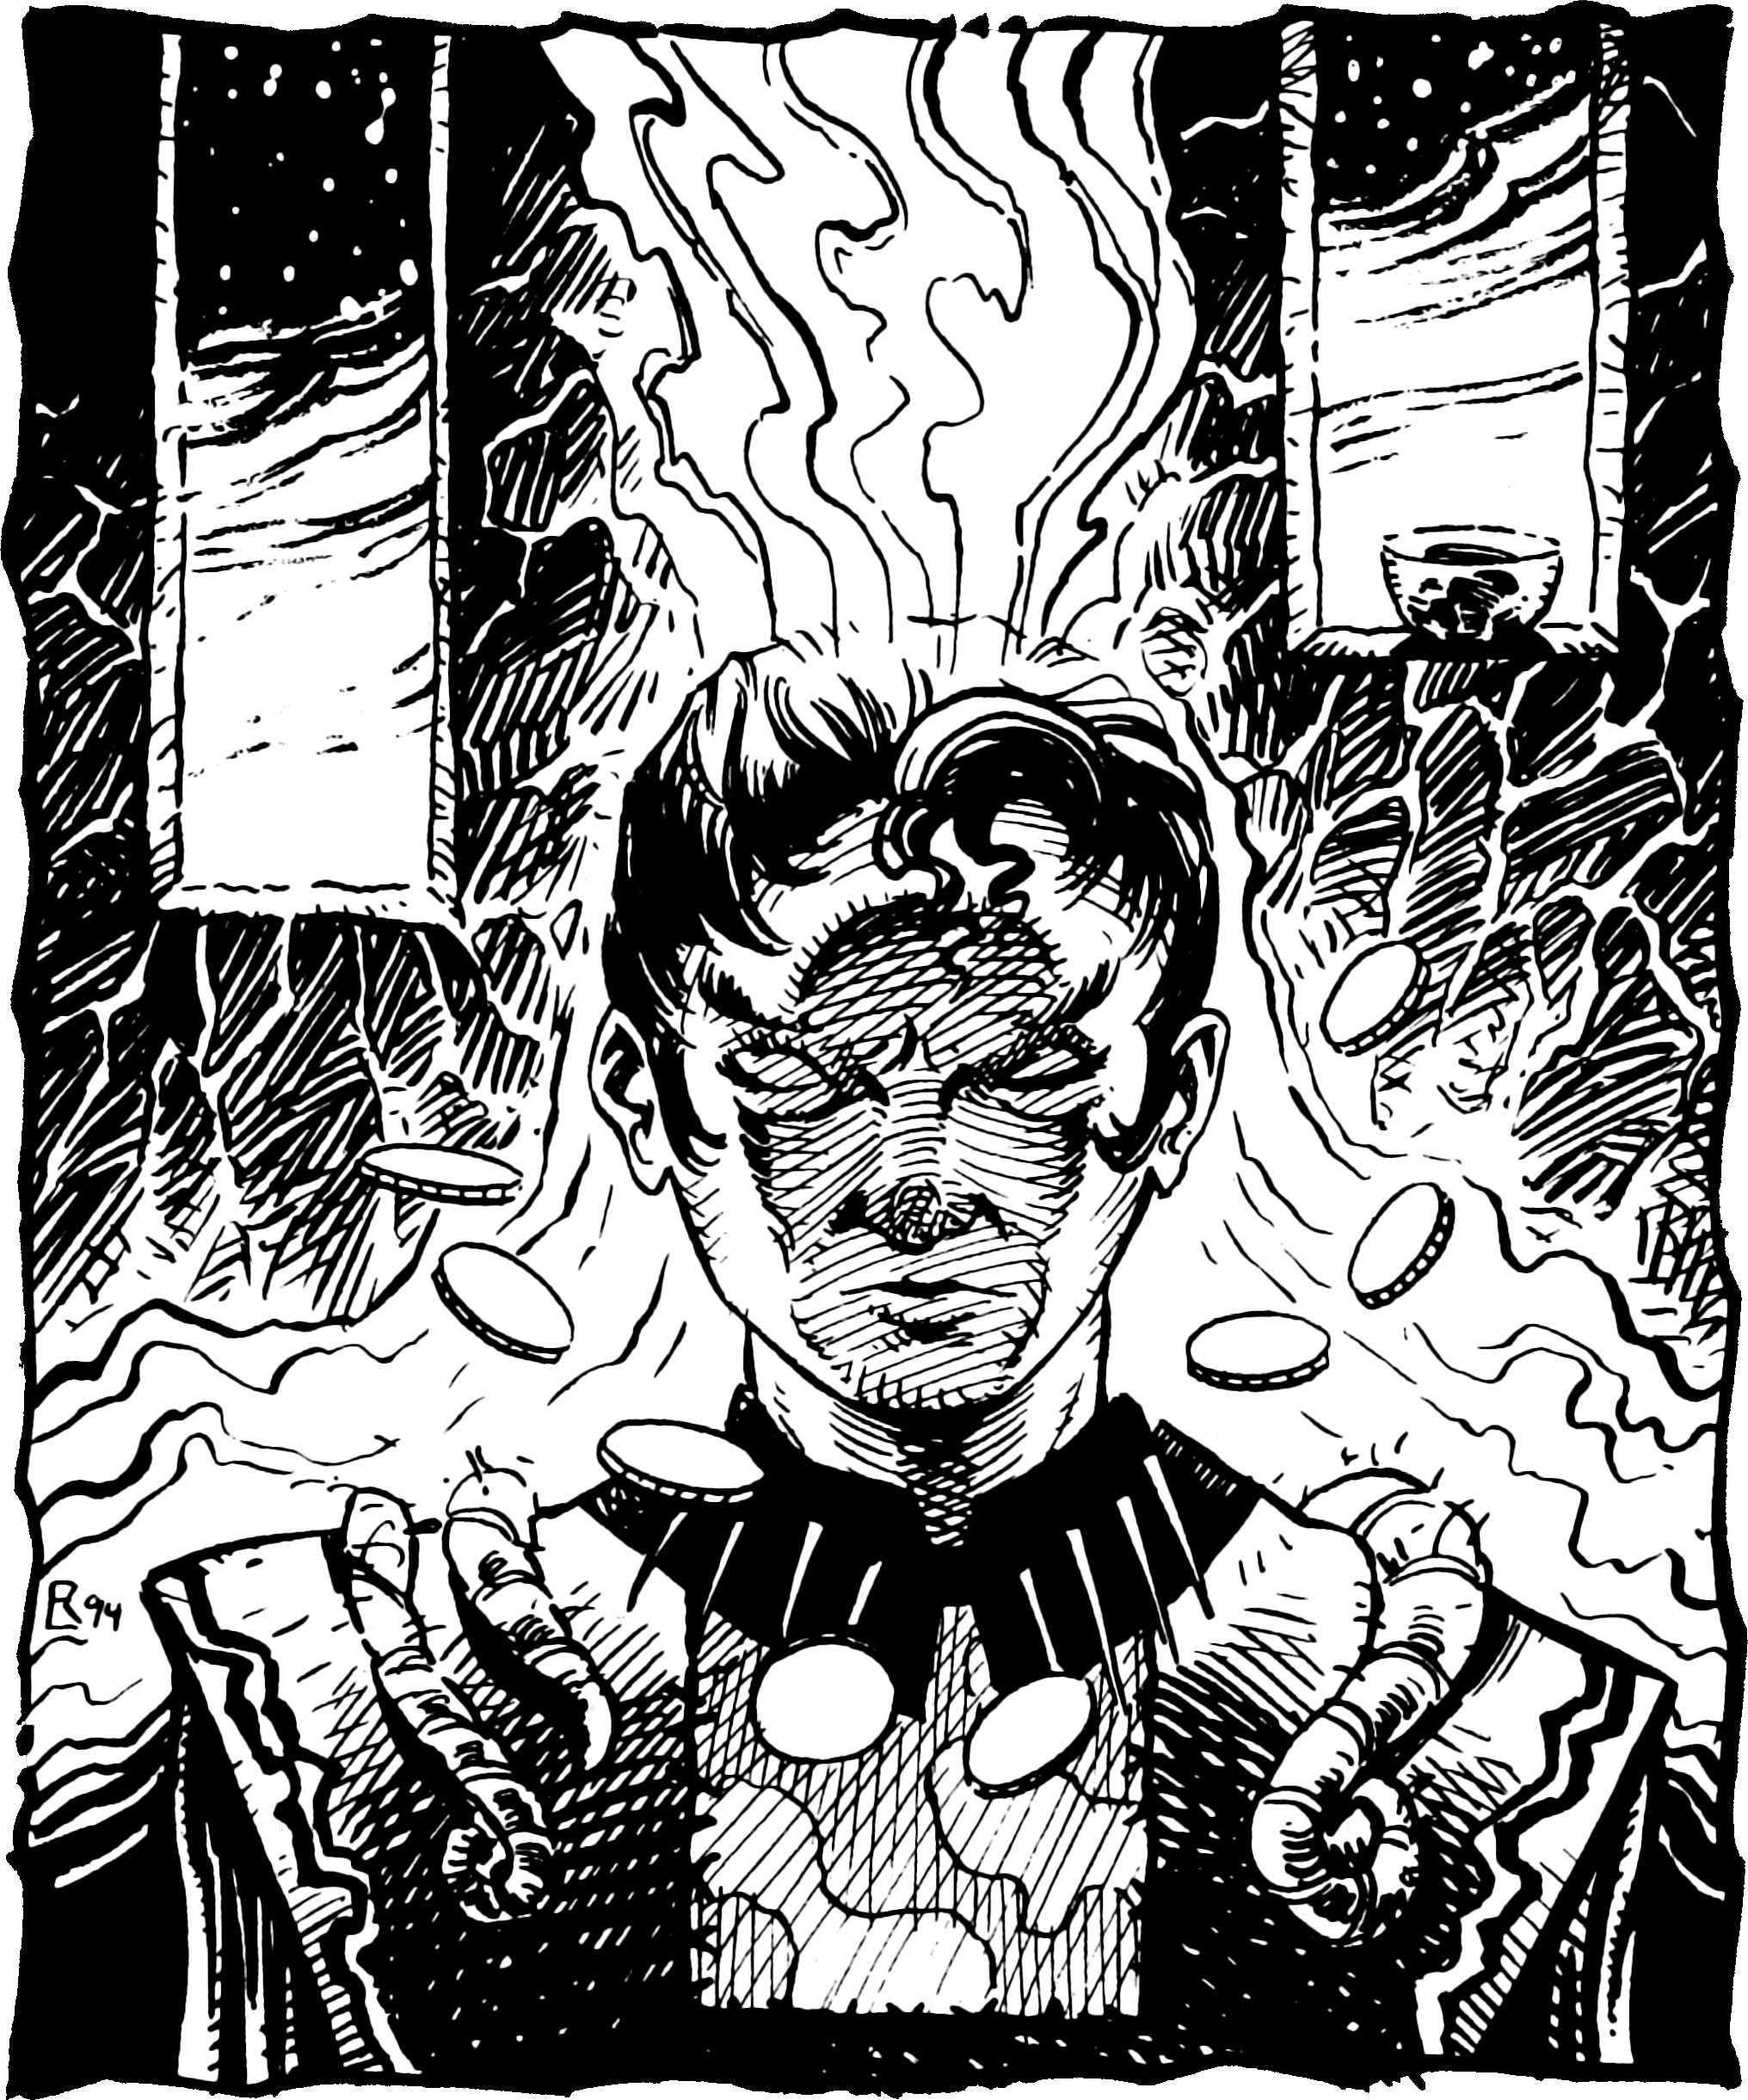
\includegraphics[width=\columnwidth]{images/psion-2.png}
\WOTC
\end{figure}

\subsection{Making a Psion}
The psion learns the Way in order to shape his Will. The psion uses, through study called the Way, how to manifest the power inherent in his inner self. The psion is able to project this power, the Will, into creating all sorts of supernatural effects. The psion may know a limited number of ways to shape his will, but he enjoys great flexibility in how he uses his known powers.

\textbf{Races:} Nearly all living creatures have a latent psionic capacity, and psions are found among all sentient races of the Tablelands, and even among some creatures that are not ordinarily considered sentient.

\textbf{Alignment:} The search for refinement of the Way tends to draw many psions into a neutral view of the world, so most psions have one part of their alignment that is neutral. Good psions may spend their time in search of new powers, or help their village defend itself against predators, or maybe join the ranks of Merchant Houses. Evil psions may serve as agents in service of the sorcerer-kings, or as more shady agents of Merchant Houses, or simply work as mercenaries and offer their specialized services to the highest bidder. Even though many psions tend to have a neutral view of the world, they can be of any alignment.

\subsection{Game Rule Information}

\textbf{Hit Die:} d4.

\subsubsection{Class Skills}

\skill{Concentration} (Con), \skill{Craft} (Int), \skill{Knowledge} (all skills, taken individually) (Int), \skill{Profession} (Wis), and \skill{Psicraft} (Int). In addition, a psion gains access to additional class skills based on his discipline:

\textbf{Seer (Clairsentience):} \skill{Gather Information} (Cha), \skill{Listen} (Wis), and \skill{Spot} (Wis).

\textbf{Shaper (Metacreativity):} \skill{Bluff} (Cha), \skill{Disguise} (Cha), and \skill{Use Psionic Device} (Cha).

\textbf{Kineticist (Psychokinesis):} \skill{Autohypnosis} (Wis), \skill{Disable Device} (Dex), and \skill{Intimidate} (Cha).

\textbf{Egoist (Psychometabolism):} \skill{Autohypnosis} (Wis), \skill{Balance} (Dex) and \skill{Heal} (Wis).

\textbf{Nomad (Psychoportation):} \skill{Climb} (Str), \skill{Jump} (Str), \skill{Ride} (Dex), \skill{Survival} (Wis), and \skill{Swim} (Str).

\textbf{Telepath (Telepathy):} \skill{Bluff} (Cha), \skill{Diplomacy} (Cha), \skill{Gather Information} (Cha), and \skill{Sense Motive} (Wis).

\textbf{Skill Points per Level:} 2 + Int modifier ($\times 4$ at 1st level).

\subsubsection{Class Features}

\textbf{Weapon and Armor Proficiency:} Psions are proficient with the club, dagger, heavy crossbow, light crossbow, quarterstaff, and shortspear. They are not proficient with any type of armor or shield. Armor does not, however, interfere with the manifestation of powers.

\textbf{Power Points per Day:} A psion's ability to manifest powers is limited by the power points he has available. His base daily allotment of power points is given on \tabref{The Psion}. In addition, he receives bonus power points per day if he has a high Intelligence score (see \tabref{Ability Scores and Bonus Power Points}). His race may also provide bonus power points per  day, as may certain feats and items.

\textbf{Discipline:} Every psion must decide at 1st level which psionic discipline he will specialize in. Choosing a discipline provides a psion with access to the class skills associated with that discipline (see above), as well as the powers restricted to that discipline. However, choosing a discipline also means that the psion cannot learn powers that are restricted to other disciplines. He can't even use such powers by employing psionic items.

\textbf{Powers Known:} A psion begins play knowing three psion powers of your choice. Each time he achieves a new level, he unlocks the knowledge of new powers.

Choose the powers known from the psion power list, or from the list of powers of your chosen discipline. You cannot choose powers from restricted discipline lists other than your own discipline list. You can choose powers from disciplines other than your own if they are not on a restricted discipline list. (Exception: The feats Expanded Knowledge and Epic Expanded Knowledge do allow a psion to learn powers from the lists of other disciplines or even other classes.) A psion can manifest any power that has a power point cost equal to or lower than his manifester level.

The number of times a psion can manifest powers in a day is limited only by his daily power points.

A psion simply knows his powers; they are ingrained in his mind. He does not need to prepare them (in the way that some spellcasters prepare their spells), though he must get a good night's sleep each day to regain all his spent power points.

The Difficulty Class for saving throws against psion powers is 10 + the power's level + the psion's Intelligence modifier. Maximum Power Level Known: A psion begins play with the ability to learn 1st-level powers. As he attains higher levels, a psion may gain the ability to master more complex powers.

To learn or manifest a power, a psion must have an Intelligence score of at least 10 + the power's level.

\textbf{Bonus Feats:} A psion gains a bonus feat at 1st level, 5th level, 10th level, 15th level, and 20th level. This feat must be a psionic feat, a metapsionic feat, or a psionic item creation feat.

These bonus feats are in addition to the feats that a character of any class gains every three levels. A psion is not limited to psionic feats, metapsionic feats, and psionic item creation feats when choosing these other feats.

\subsubsection{Psionic Disciplines}
A discipline is one of six groupings of powers, each defined by a common theme. The six disciplines are clairsentience, metacreativity, psychokinesis, psychometabolism, psychoportation, and telepathy.

\textbf{Clairsentience:} A psion who chooses clairsentience is known as a seer. Seers can learn precognitive powers to aid their comrades in combat, as well as powers that permit them to gather information in many different ways.

\textbf{Metacreativity:} A psion specializing in metacreativity is known as a shaper. This discipline includes powers that draw ectoplasm or matter from the Astral Plane, creating semisolid and solid items such as armor, weapons, or animated constructs to do battle at the shaper's command.

\textbf{Psychokinesis:} Psions who specialize in psychokinesis are known as kineticists. They are the masters of powers that manipulate and transform matter and energy. Kineticists can attack with devastating blasts of energy.

\textbf{Psychometabolism:} A psion who specializes in psychometabolism is known as an egoist. This discipline consists of powers that alter the psion's psychobiology, or that of creatures near him. An egoist can both heal and transform himself into a fearsome fighter.

\textbf{Psychoportation:} A psion who relies on psychoportation powers is known as a nomad. Nomads can wield powers that propel or displace objects in space or time.

\textbf{Telepathy:} A psion who chooses the discipline of telepathy is known as a telepath. He is the master of powers that allow mental contact and control of other sentient creatures. A telepath can deceive or destroy the minds of his enemies with ease.

\subsubsection{Psicrystals}

\begin{figure}[t!]
\centering
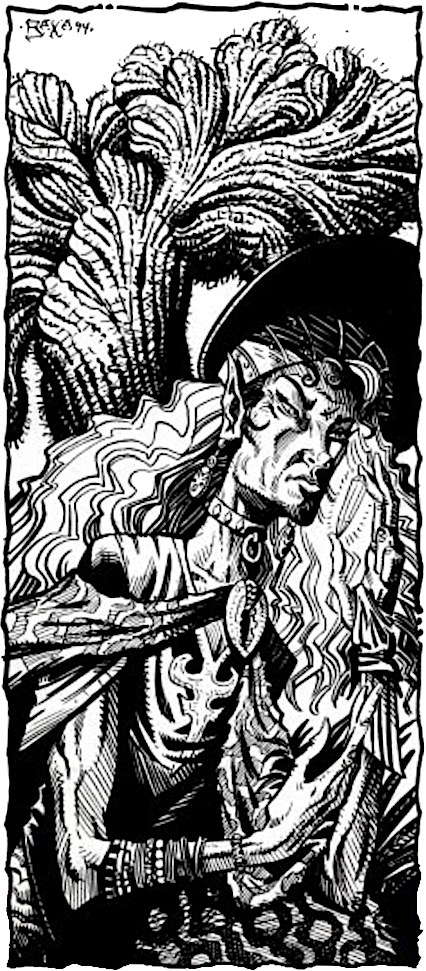
\includegraphics[width=\columnwidth-2mm]{images/psion-3.png}
\WOTC
\end{figure}

A psicrystal is a fragment of a psionic character's personality, brought into physical form and a semblance of life (via the \feat{Psicrystal Affinity} feat). A psicrystal appears as a crystalline construct about the size of a human hand.

Because it is an extension of its creator's personality, a character's psicrystal is in some ways a part of him. That's why, for example, a psionic character can manifest a personal range power on his psicrystal even though normally he can manifest such a power only on himself.

A psicrystal is treated as a construct for the purposes of all effects that depend on its type.

A psicrystal grants special abilities to its owner, as shown on the \tabref{Psicrystal Special Abilities}. In addition, a psicrystal has a personality (being a fragment of the owner's personality), which gives its owner a bonus on certain types of checks or saving throws, as given on the Psicrystal Personalities table below. These special abilities and bonuses apply only when the owner and the psicrystal are within 1.5 kilometer of each other.

Psicrystal abilities are based on the owner's levels in psionic classes. Levels from other classes do not count toward the owner's level for purposes of psicrystal abilities.

A psicrystal can speak one language of its owner's choice (so long as it is a language the owner knows). A psicrystal can understand all other languages known by its owner, but cannot speak them. This is a supernatural ability.

\textbf{Psicrystal Basics:} Use the statistics for a psicrystal, but make the following changes.

\textit{Saving Throws:} A psicrystal uses its owner's base saving throw bonuses and ability modifiers on saves, though it doesn't enjoy any other bonuses its owner might have (from magic items or feats, for example).

\textit{Abilities:} When its self-propulsion ability is not activated, a psicrystal has no Strength score and no Dexterity score.

\textit{Skills:} A psicrystal has the same skill ranks as its owner, except that it has a minimum of 4 ranks each in \skill{Spot}, \skill{Listen}, \skill{Move Silently}, and \skill{Search}. (Even if its owner has no ranks in these skills, a psicrystal has 4 ranks in each.) A psicrystal uses its own ability modifiers on skill checks.

\Table{Psicrystal Special Abilities}{X C Z{1cm} b{4.2cm}} {
\tableheader Owner Level & \tableheader Natural Armor Adj. & \tableheader Int Adj. & \tableheader Special \\
1--2 & +0 & +0 & Alertness, improved evasion, personality, self-propulsion, share powers, sighted, telepathic link \\
3--4 & +1 & +1 & Deliver touch powers \\
5--6 & +2 & +2 & Telepathic speech \\
7--8 & +3 & +3 &\\
9--10 & +4 & +4 & Flight \\
11--12 & +5 & +5 & Power resistance \\
13--14 & +6 & +6 & Sight link \\
15--16 & +7 & +7 & Channel power \\
17--18 & +8 & +8 &\\
19--20 & +9 & +9 &
}

\textbf{Psicrystal Ability Descriptions:} All psicrystals have special abilities (or impart abilities to their owners) depending on the level of the owner, as shown on the table above. The abilities on the table are cumulative.

\textit{Natural Armor Adj. (Ex):} This number noted here is an improvement to the psicrystal's natural armor bonus (normally 0). It represents a psicrystal's preternatural durability.

\textit{Intelligence Adj. (Ex):} Add this value to the psicrystal's Intelligence score. Psicrystals are as smart as people (though not necessarily as smart as smart people).

\textit{Alertness (Ex):} The presence of a psicrystal sharpens its master's senses. While a psicrystal is within arm's reach (adjacent to or in the same square as its owner), its owner gains the Alertness feat.

\textit{Improved Evasion (Ex):} If a psicrystal is subjected to an attack that normally allows a Reflex saving throw for half damage, it takes no damage if it makes a successful saving throw and half damage even if the saving throw fails.

\textit{Personality (Ex):} Every psicrystal has a personality. See Psicrystal Personality, below.

\textit{Self-Propulsion (Su):} As a standard action, its owner can will a psicrystal to form spidery, ectoplasmic legs that grant the psicrystal a land speed of 9 meters and a climb speed of 6 meters. The legs fade into nothingness after one day (or sooner, if the owner desires).

\textit{Share Powers (Su):} At the owner's option, he can have any power (but not any psi-like ability) he manifests on himself also affect his psicrystal. The psicrystal must be within 1.5 meter of him at the time of the manifestation to receive the benefit. If the power has a duration other than instantaneous, it stops affecting the psicrystal if it moves farther than 1.5 meter away, and will not affect the psicrystal again, even if it returns to its owner before the duration expires.

Additionally, the owner can manifest a power with a target of ``You'' on his psicrystal (as a touch range power) instead of on himself. The owner and psicrystal cannot share powers if the powers normally do not affect creatures of the psicrystal's type (construct).

\textit{Sighted (Ex):} Although it has no physical sensory organs, a psicrystal can telepathically sense its environment as well as a creature with normal vision and hearing. Darkness (even supernatural darkness) is irrelevant, as are areas of supernatural silence, though a psicrystal still can't discern invisible or ethereal beings. A psicrystal's sighted range is 12 meters.

\textit{Telepathic Link (Su):} The owner has a telepathic link with his psicrystal out to a distance of up to 1.5 kilometer. The owner cannot see through the psicrystal's senses, but the two of them can communicate telepathically as if the psicrystal were the target of a mindlink power manifested by the owner. For instance, a psicrystal placed in a distant room could relay the activities occurring in that room.

Because of the telepathic link between a psicrystal and its owner, the owner has the same connection to an item or place that the psicrystal does. For instance, if his psicrystal has seen a room, the owner can teleport into that room as if he has seen it too.

\textit{Deliver Touch Powers (Su):} If the owner is 3rd level or higher, his psicrystal can deliver touch powers for him. If the owner and psicrystal are in contact at the time the owner manifests a touch power, he can designate his psicrystal as the ``toucher.'' The psicrystal can then deliver the touch power just as the owner could. As usual, if the owner manifests another power before the touch is delivered, the touch power dissipates.

\textit{Telepathic Speech (Ex):} If the owner is 5th level or higher, the psicrystal can communicate telepathically with any creature that has a language and is within 9 meters of the psicrystal, while the psicrystal is also within 1.5 kilometer of the owner.

\textit{Flight (Su):} If the owner is 9th level or higher, he can, as a standard action, will his psicrystal to fly at a speed of 15 meters (poor). The psicrystal drifts gently to the ground after one day (or sooner, if the owner desires).

\textit{Power Resistance (Ex):} If the owner is 11th level or higher, the psicrystal gains power resistance equal to the owner's level + 5. To affect the psicrystal with a power, another manifester must get a result on a manifester level check that equals or exceeds the psicrystal's power resistance.

\textit{Sight Link (Sp):} If the owner is 13th level or higher, the character can remote view the psicrystal (as if manifesting the remote view power) once per day.

\textit{Channel Power (Sp):} If the owner is 15th level or higher, he can manifest powers through the psicrystal to a distance of up to 1.5 kilometer. The psicrystal is treated as the power's originator, and all ranges are calculated from its location.

When channeling a power through his psicrystal, the owner manifests the power by paying its power point cost. He is still subject to attacks of opportunity and other hazards of manifesting a power, if applicable (for instance, he becomes visible when manifesting an offensive power if invisible, as does the psicrystal).

\Table{Psicrystal Personalities}{b{2cm} X}{
\tableheader Personality & \tableheader Benefit to Owner\\
Artiste & +3 bonus on \skill{Craft} checks\\
Bully & +3 bonus on \skill{Intimidate} checks\\
Coward & +3 bonus on \skill{Hide} checks\\
Friendly & +3 bonus on \skill{Diplomacy} checks\\
Hero & +2 bonus on Fortitude saves\\
Liar & +3 bonus on \skill{Bluff} checks\\
Meticulous & +3 bonus on \skill{Search} checks\\
Nimble & +2 bonus on Initiative checks\\
Observant & +3 bonus on \skill{Spot} checks\\
Poised & +3 bonus on \skill{Balance} checks\\
Resolved & +2 bonus on Will saves\\
Sage & +3 bonus on checks involving any one \skill{Knowledge} skill owner already knows; once chosen, this does not vary\\
Single-minded & +3 bonus on \skill{Concentration} checks\\
Sneaky & +3 bonus on \skill{Move Silently} checks\\
Sympathetic & +3 bonus on \skill{Sense Motive} checks
}

\textbf{Psicrystal Personality (Ex):} Each psicrystal has a distinct personality, chosen by its owner at the time of its creation from among those given on the following table. At 1st level, its owner typically gets a feel for a psicrystal's personality only through occasional impulses, but as the owner increases in level the psicrystal's personality becomes more pronounced. At higher levels, it is not uncommon for a psicrystal to constantly ply its owner with observations and advice, often severely slanted toward the psicrystal's particular worldview. The owner always sees a bit of himself in his psicrystal, even if magnified and therefore distorted.

\subsection{Playing a Psion}
When you first learned to use psionics, you were taught to create a nexus---a point in the center of your being where physical, mental, and spiritual energy can be harnessed. It is the union of these powers that allows you to perform the remarkable feats you're capable of.

As a psion, your choice of discipline is all-important to you. Seers are not very powerful, if one defines power as the ability to cause immediate harm to one's foes, but they are the most capable information gatherers of Athas. Shapers are tinkerers, creating toys and monsters out of thin air, just to dismiss them and build another. Kineticists are battlefield psionicists who are actively sought out as military auxiliaries, and is almost as good as a wizard for creating mayhem in a fight. Egoists have a wide range of useful powers: they can fight as well as a fighter, become stealthier than a thief, heal like a cleric, or change shape like a wizard. Nomads possess an array of valuable powers that can bypass almost any obstacle and confound any enemies, working with the very fabric of space, time, and reality itself to achieve his goals. Telepaths are considered by some to the most powerful psions, and most Athasians are terrified of a telepath's ability to manipulate their very thoughts.

\subsubsection{Religion}
Psions use the Way to manifest their inner powers; through long hours of meditation and extremes of the senses, they seek knowledge inward. Their power comes from inside them, so only psions from the most animistic cultures look to outside beings or religions for spiritual fulfillment.

\subsubsection{Other Classes}
Psions tend to be drawn to those like themselves. Lower-level psions tend to towards a nearly worshipful attitude towards higher level psions, curious about their mysterious training and knowledge.

Higher-level psions tend to either stay to themselves, or to try to befriend almost everyone, pressing for party leadership. Most psions tolerate priests and druids (although some psions make needling remarks about ``foolish superstition''), but most psions are uneasy with wizards. Psions view wilders much in the same way that a fighter views a barbarian---untrained, erratic, and as much a danger to his companions as to his enemies.

\subsubsection{Combat}

You usually disdain combat and other primitive displays of force, but when needed, you use your impressive array of psionic powers for both attack and defense against your enemies, just as any other psionic character would.

\subsubsection{Advancement}

Most psions were strongly inclined towards a specific discipline before their ever realized they had any psionic talent. Once you have undergone your initial training, you can continue your studies on your own, much the way a wizard learn new spells.

As you attain more levels in the psion class, the most important choice you face is which powers to learn. A psion has access to much fewer spells than a wizard, so he has to chose carefully in order to find a good mix of offensive, defensive, and utility powers.

\subsection{Starting Packages}
\subsubsection{The Blaster}

Aarakocra Psion (Kineticist)

\textbf{Ability Scores:} Str 8, Dex 18, Con 13, Int 15, Wis 12, Cha 6.

\textbf{Skills:} \skill{Concentration}, \skill{Intimidate}, \skill{Knowledge} (psionics), \skill{Psicraft}.

\textbf{Languages:} Auran, Common.

\textbf{Feat:} \feat{Overchannel}.

\textbf{Weapons:} Shortspear (1d6, 6 m)

Light crossbow with 20 bolts (1d6/19--20, 24 m).

\textbf{Armor:} None.

\textbf{Other Gear:} Standard adventurer's kit, 62 cp.

\subsubsection{The Mindbender}
Human Psion (Telepath)

\textbf{Ability Scores:} Str 8, Dex 10, Con 12, Int 15, Wis 13, Cha 14.

\textbf{Skills:} \skill{Bluff}, \skill{Concentration}, \skill{Gather Information}, \skill{Knowledge} (local), \skill{Sense Motive}.

\textbf{Languages:} Common.

\textbf{Feat:} \skill{Inquisitor}, \skill{Psionic Endowment}.

\textbf{Weapons:} Club (1d4)

Light crossbow with 20 bolts (1d6/19--20, 24 m).

\textbf{Armor:} None.

\textbf{Other Gear:} Standard adventurer's kit, 63 cp.

\subsubsection{The Teleporter}
Elf Psion (Nomad)

\textbf{Ability Scores:} Str 10, Dex 16, Con 10, Int 15, Wis 13, Cha 8.

\textbf{Skills:} \skill{Concentration}, \skill{Jump}, \skill{Psicraft}, \skill{Survival}.

\textbf{Languages:} Elven, Common.

\textbf{Feat:} \feat{Speed of Thought}.

\textbf{Weapons:} Quarterstaff (1d6)

Dagger (1d4/19--20, 3 m)

Shortbow with 20 arrows (1d6/$\times$3. 18 m).

\textbf{Armor:} None.

\textbf{Other Gear:} Standard adventurer's kit, 64 cp.

% \vskip5cm
\subsection{Psions on Athas}
\Quote{Once, I encountered a shattered tribe of elves wandering aimlessly through the desert. Lost and unprovisioned, they clearly had no hope of survival beyond the next few days. I later learned that they had made the mistake of disturbing a psionic master's trance as they attempted to rob his home.}{The Wanderer's Journal}

Nearly every level of Athasian society is permeated with psionics. Even the humblest slave may possess an unusual talent or ability, while the most powerful enchantments of the sorcerer-monarchs include psionic elements. Mental powers are used on an everyday basis in Athasian culture.

Telepaths allow instantaneous communication across hundreds of miles. Draft animals and slaves are kept under control by psionic overseers. Prophets use their visionary powers to forecast the fortunes of kings and peasants, find missing objects, and solve crimes. Kineticists and egoists use their potent abilities in all manner of enterprises, both legitimate and otherwise.

\subsubsection{Daily Life}

The study of the Way is very similar to the study of magic. Just as wizards strive to master more advanced and difficult spells, psionicists must constantly seek to unlock new and more powerful abilities. Unlike wizardry, there is no single formula that will reproduce an effect of the Way that will work the same for each individual. Students must independently develop the command of their powers.

High-level psions tend to become contemplative masters, so they can make good patrons for lower-level PCs. Such psions often hire adventurers to gather rare psionic items for study or to recover lost knowledge of the ancient ages in their stead.

\subsubsection{Notables}

The human psion known as Pharistes brought chaos over the Tyr Region when he activated a powerful artifact that dampened all psionic power in the region and drove all thri-kreen mad because he thought the abuse of psionics was the cause of all the evil under the dark sun. Agis of Asticles was an accomplished telepath and politician, who fought to bring freedom to the city-stated of Tyr and helped to remove Athas from the menace of the Dragon of Tyr.

\subsubsection{Organizations}

Psions don't organize together, but they often join other organizations, specially psionic academies and monasteries. Psions who dedicate themselves into extensive studies in such organizations in order to master the Way often become \class{Psiologists}.

\subsubsection{NPC Reactions}

The common people usually react to a psion exactly as they would to any other psionicists in their community. Because trained psionicists are scarce and their skills are vital, they are highly valued by many elements of the Athasian society. Unlike wizards, psionicists are free of the taint of magic and need not disguise their calling. They owe no loyalty to the sorcerer-kings, unlike the templars. Even clerics and druids have elemental powers and guarded lands that they must place before all other considerations. Psionicists are free of these patrons and responsibilities and may employ their powers as they see fit.

\subsubsection{Psion Lore}

Characters with ranks in \skill{Knowledge} (psionics) can research psions to learn more about them. When a character makes a skill check, read or paraphrase the following, including the information from lower DCs.

\textbf{DC 10:} Psions are manifesters who use the forces of their own minds to affect their environment.

\textbf{DC 15:} Psionic powers do not draw upon magical energy that surrounds all things. Rather they are derived from within when the psionicist has his entire essence in coordination; his mind, body, and soul in perfect harmony.

\textbf{DC 20:} Psions choose one of the six psionic disciplines in which to focus their efforts.
